\section{Ruby on Rails} % (fold)
\label{tech:sec:ruby_on_rails}
David Hansson began developing a web-based project management tool oriented towards small teams in 2003. Working at \textit{37signals}, he initially started by using PHP but soon became frustrated by many of the language's shortcomings. He gave up on this language and started implementing what today is known as \textit{Basecamp} in pure Ruby. While developing the application, he noticed that a lot of its code could be extracted into a framework for future use with other applications. Hansson decided to release his framework to the public in July 2004 and Ruby on Rails was born~\cite{railssolutions}.

Rails started to become more mature over time and applications like Twitter, YellowPages, Hulu, Scribd and GitHub were built using this framework. Its popularity has grown significantly since the beginning and its adoption by popular platforms helped establishing Rails as a solid framework.

Ruby on Rails has three main principles behind its creation~\cite{agile_webdevelopment_with_rails, ruby_on_rails_principles}:
\begin{description}
\item[Convention over configuration.] In Rails, everything has a default configuration. The only exception is the database connection data. This way, developers only need to specify when they want to use unconventional configurations. This way, Rails offers simplicity while retaining high flexibility.
\item[Don't Repeat Yourself.] Also known as DRY, this practice implies that the similar code snippets do not exist in separate locations. Every piece of knowledge is unique, definite and has a relevant representation. This simplifies modifications by the avoidance of having to change the same logic in different parts of the project, allowing the applications to keep a high consistency degree.
\item[Model-View-Controller.] Rails follows the MVC architecture pattern, keeping the source code well organized by clearly separating the code according to its purpose. The \textit{Model} is responsible for maintain the state of the application, specifying the constraints its related data has to obey to. The \textit{Controller} receives the users' input, interacts with the model and finally renders a view page as the result. The \textit{View} can have multiple formats, from JSON to XML, and is essentially what is displayed to the users. This principle's schema is presented in figure~\ref{fig:mvc}.
\begin{figure}[h]
  \centering
  \caption{Model-View-Controller Architectural Pattern}
  \label{fig:mvc}
    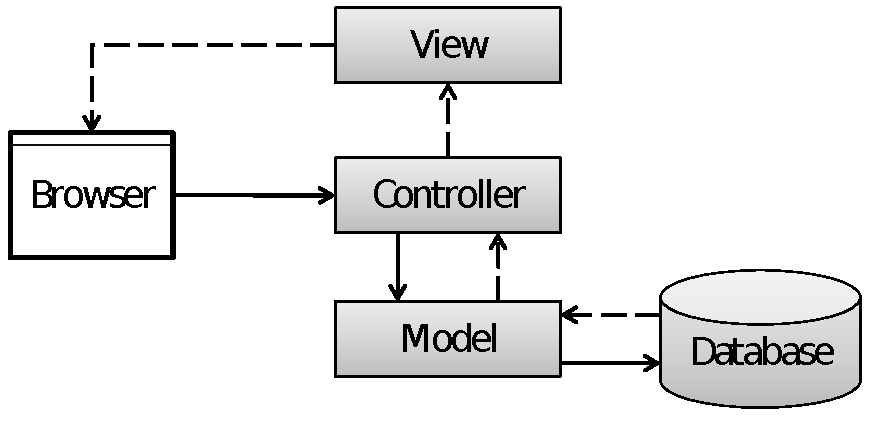
\includegraphics[width=0.75\textwidth]{mvc}
\end{figure}\\
\end{description}
Rails' functionality can be altered and extended with \textit{plugins} and \textit{gems}. While being a full stack web framework, Rails does not aim to include every single feature. However, it has been built with a highly extensible infrastructure and it has a considerably large set of \textit{plugins} and compatible \textit{gems} nowadays~\cite{rails_magazine_1}.


\subsection{Rails 2}
\label{tech:sec:ruby_on_rails:rails2}
Rails 2 was first released in 2007. Its current version is 2.3, released at the beginning of 2009. Throughout these 2 years the framework was improved by many contributors, aside from the core team~\cite{rails_core_team}. The framework is essentially divided in six essential modules~\cite{ruby_on_rails_principles, rails23_release_notes}:
\begin{description}
\item[ActionPack] splits the response in two:  a request for the controller to handle and a template rendering part for the view to control.
\item[ActiveRecord] is responsible for object handling and their database representations. Objects are directly linked to the database, so modifying them will modify the table definition they are associated with.
\item[ActiveResource] corresponds to objects that represent the application's RESTful resources as manipulatable Ruby objects.
\item[ActiveSupport] is a collection of various utility classes and standard library extensions.
\item[ActionMailer] is a framework for designing email-service layers, allowing the application to send emails using a mailer model and views.
\end{description}
Having a considerable amount of modules and classes, Rails is structured according to the aforementioned components.


\subsection{Rails 3}
\label{tech:sec:ruby_on_rails:rails3}
Rails 3 is currently in development and it is on its first release candidate, after four beta versions. Most of Rails' code has been refactored and this release's main goals were concerned with improved component decoupling and performance~\cite{rails3_great_decoupling}. 

As of component decoupling, a great deal of work has been done and impressive goals have been achieved~\cite{vaporware_to_awesome}. Most of Rails' components are agnostic now, having standard interfaces for communication with each other. The key concept is that a component is agnostic to whom it is interacting with. This allows component swapping, enabling the replacement of one or more of Rails' core components with a different, third-party one. In order to make this happen standard procedures have been developed, providing standard interfaces for each one of Rails' components.

The decoupling process also allowed for improved modularity, permitting Rails' component separation. ActionController, for instance, has been split into ActionDispatch, ActionController and AbstractController~\cite{vaporware_to_awesome}. There was a lot of work on explicitly handling each component's internal dependencies. This enables the developer to carefully select which modules he needs in his Rails application without caring about including the modules it depends on as well. In previous versions of Rails developers would import the top-level modules, since the alternative was to parse the source code of the framework to find its internal dependencies in order to import all necessary modules. Applications now have the possibility to only load the modules they really need thus becoming faster and lighter.

This improved modularity also had its impact on performance. However, the team also made a specific effort into improving common Rails bottlenecks like partial and collection rendering~\cite{vaporware_to_awesome}, among some other optimized sections.

